\documentclass[11pt,a4paper]{article}
\usepackage[margin=2.2cm]{geometry}
\usepackage{booktabs}
\usepackage{graphicx}
\usepackage{amsmath}
\usepackage{float}
\usepackage[hidelinks]{hyperref}

\title{Assignment 5: Explainable AI}
\author{}
\date{}

\begin{document}
\maketitle
\vspace{-1.5cm}

All experiments use a ResNet-like model (575k parameters) trained on CIFAR-10 for 15 epochs, reaching 87.7\% test accuracy. The same trained model is reused across all four parts.

\section{Part A: Occlusion Sensitivity}

We implemented occlusion sensitivity from scratch by sliding a $4\times4$ black patch across each $32\times32$ image with stride 2 and recording the drop in predicted-class confidence. Regions where occlusion causes a large confidence drop are important for the prediction.

\begin{figure}[H]
\centering
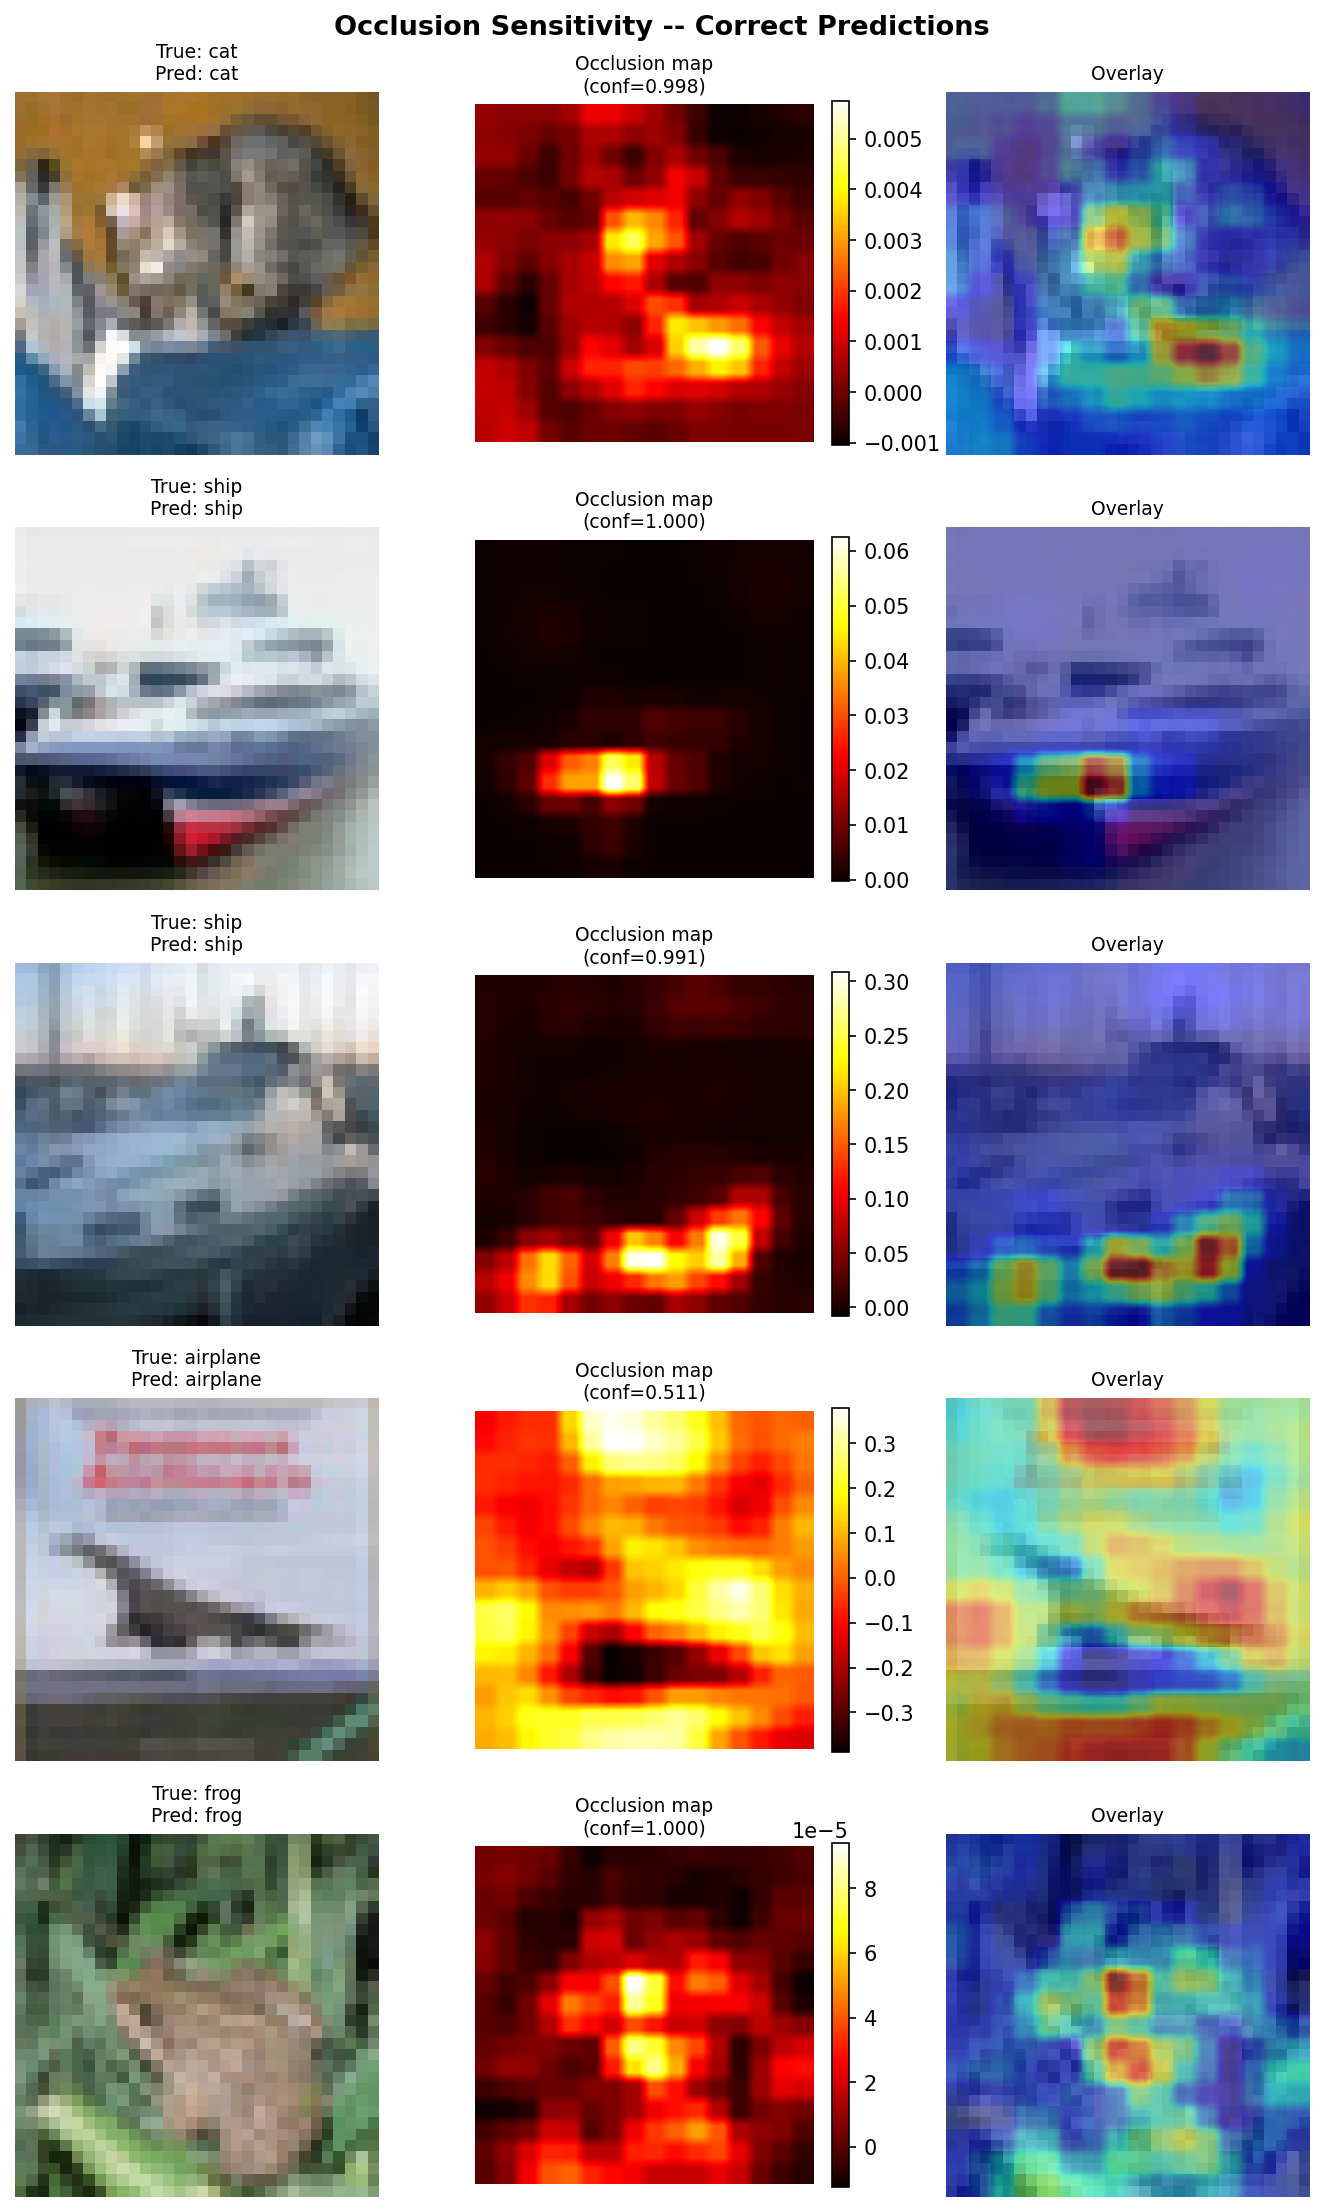
\includegraphics[width=0.85\textwidth]{occlusion_correct.png}
\caption{Occlusion heatmaps for correctly classified images. Hot regions indicate areas whose removal most reduces confidence.}
\end{figure}

For correct predictions, the heatmaps highlight the object itself -- the model's confidence drops most when the patch covers the subject (e.g., occluding a horse's body or a ship's hull). Background occlusion has minimal effect, confirming the model attends to semantically relevant regions.

\begin{figure}[H]
\centering
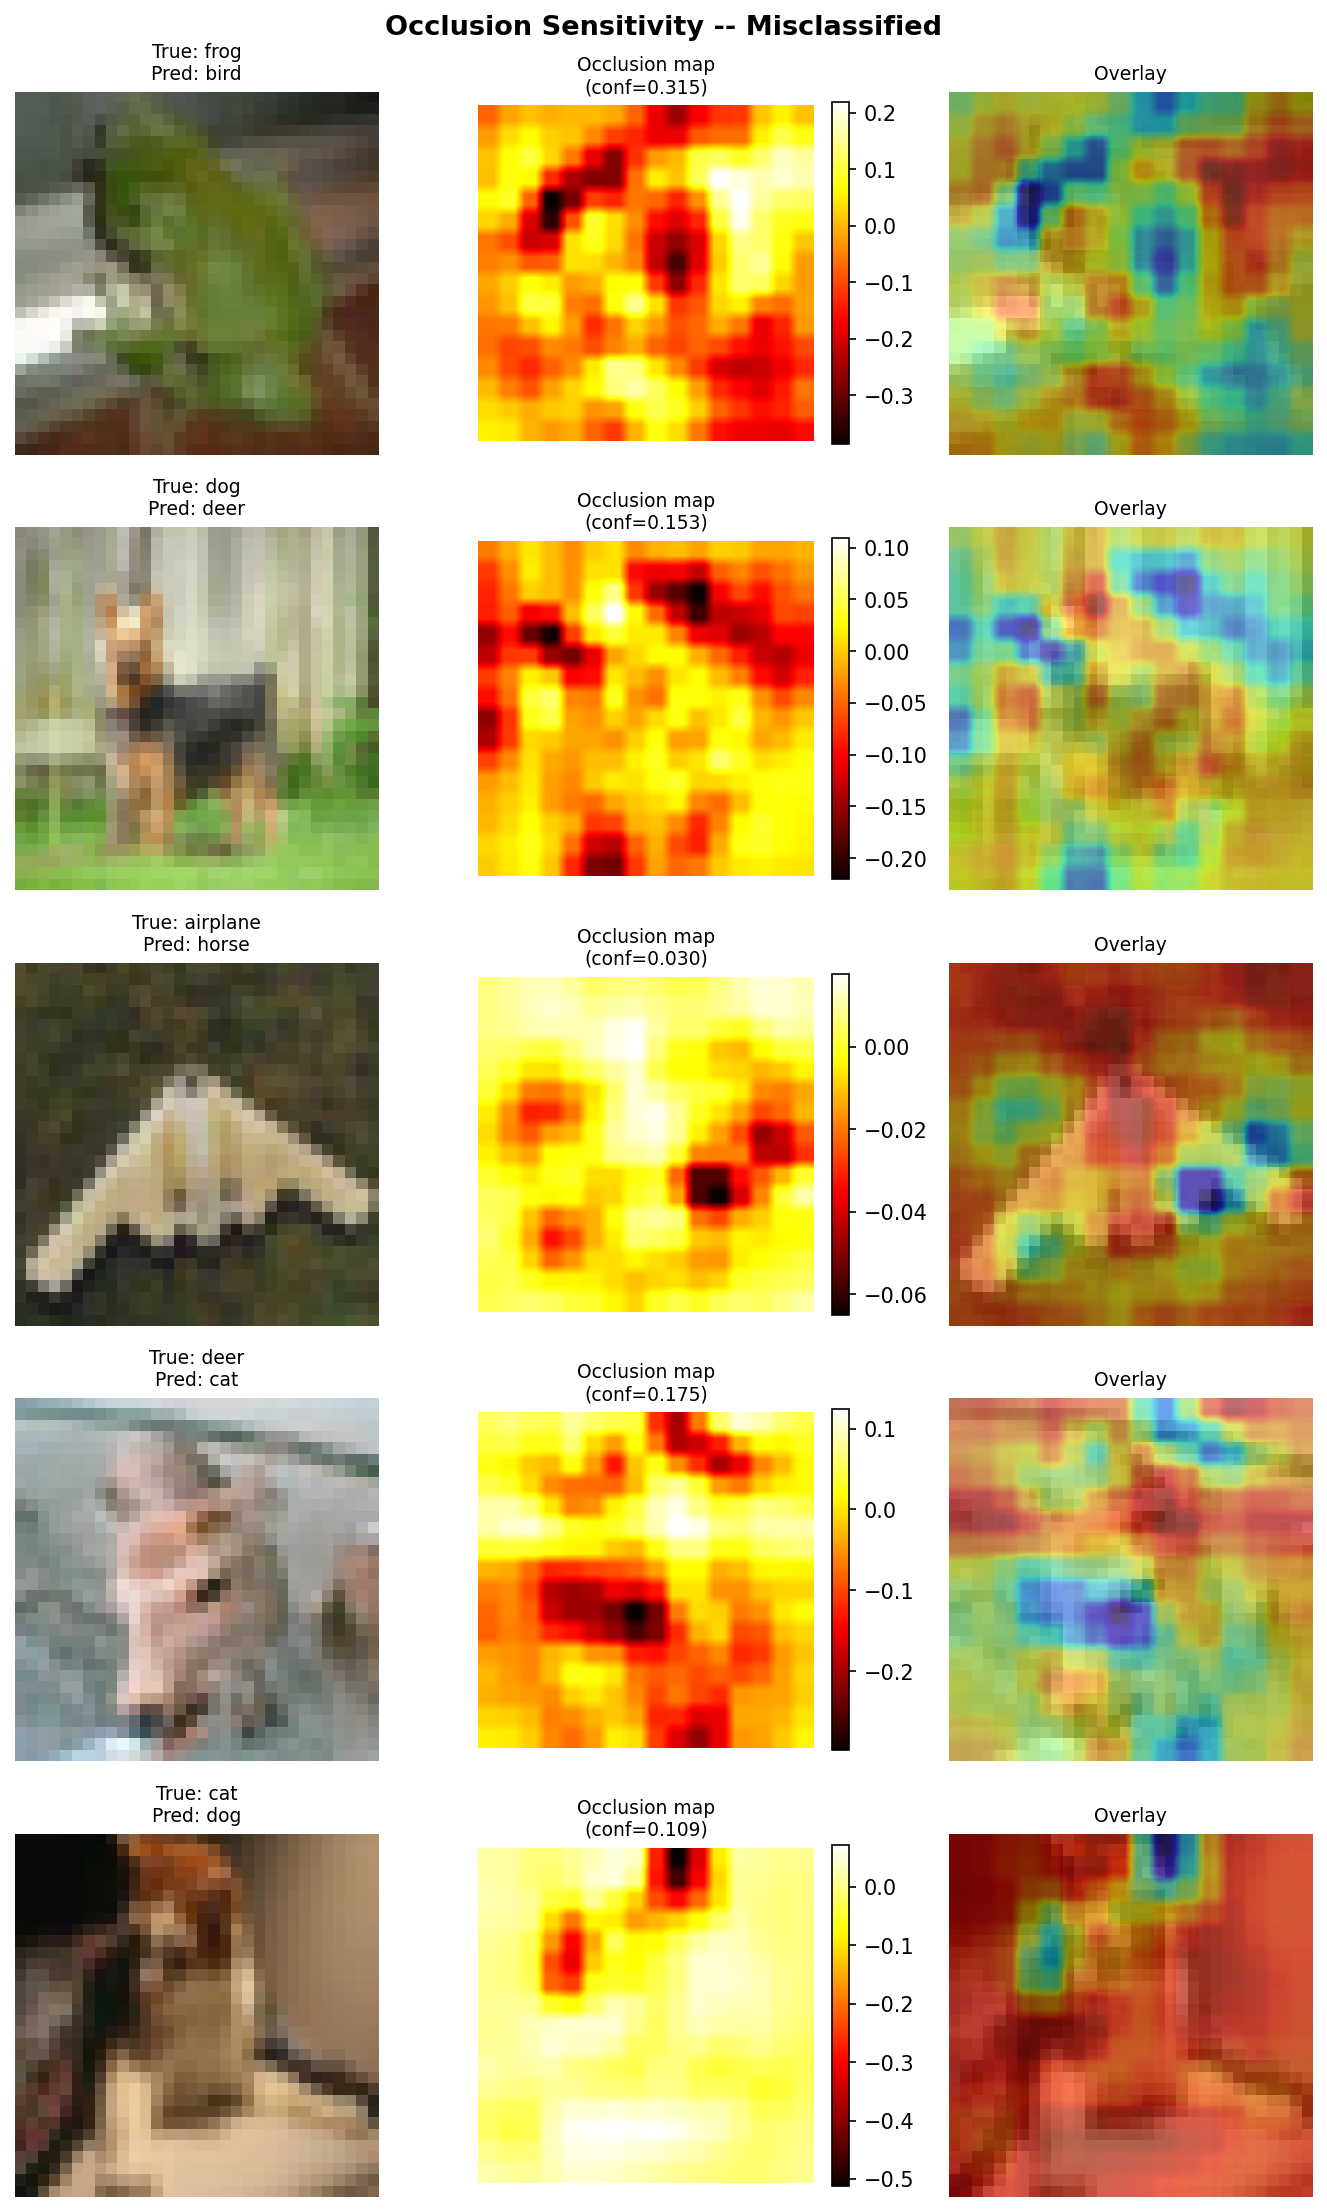
\includegraphics[width=0.85\textwidth]{occlusion_incorrect.png}
\caption{Occlusion heatmaps for misclassified images.}
\end{figure}

For misclassified images, the heatmaps reveal two patterns: either the model focuses on background regions (indicating it bases its prediction on context rather than the object), or the heatmap is diffuse with no strong focus, suggesting the model lacks a clear discriminative signal. This demonstrates that occlusion sensitivity can diagnose \emph{why} a model fails, not just \emph{that} it fails.

\section{Part B: Grad-CAM}

We applied Grad-CAM using the \texttt{pytorch-grad-cam} library, targeting the last convolutional layer (\texttt{stage3.conv2}). Grad-CAM computes the gradient of the predicted class score with respect to the feature maps, then weights each map by its average gradient to produce a class-specific activation heatmap.

\begin{figure}[H]
\centering
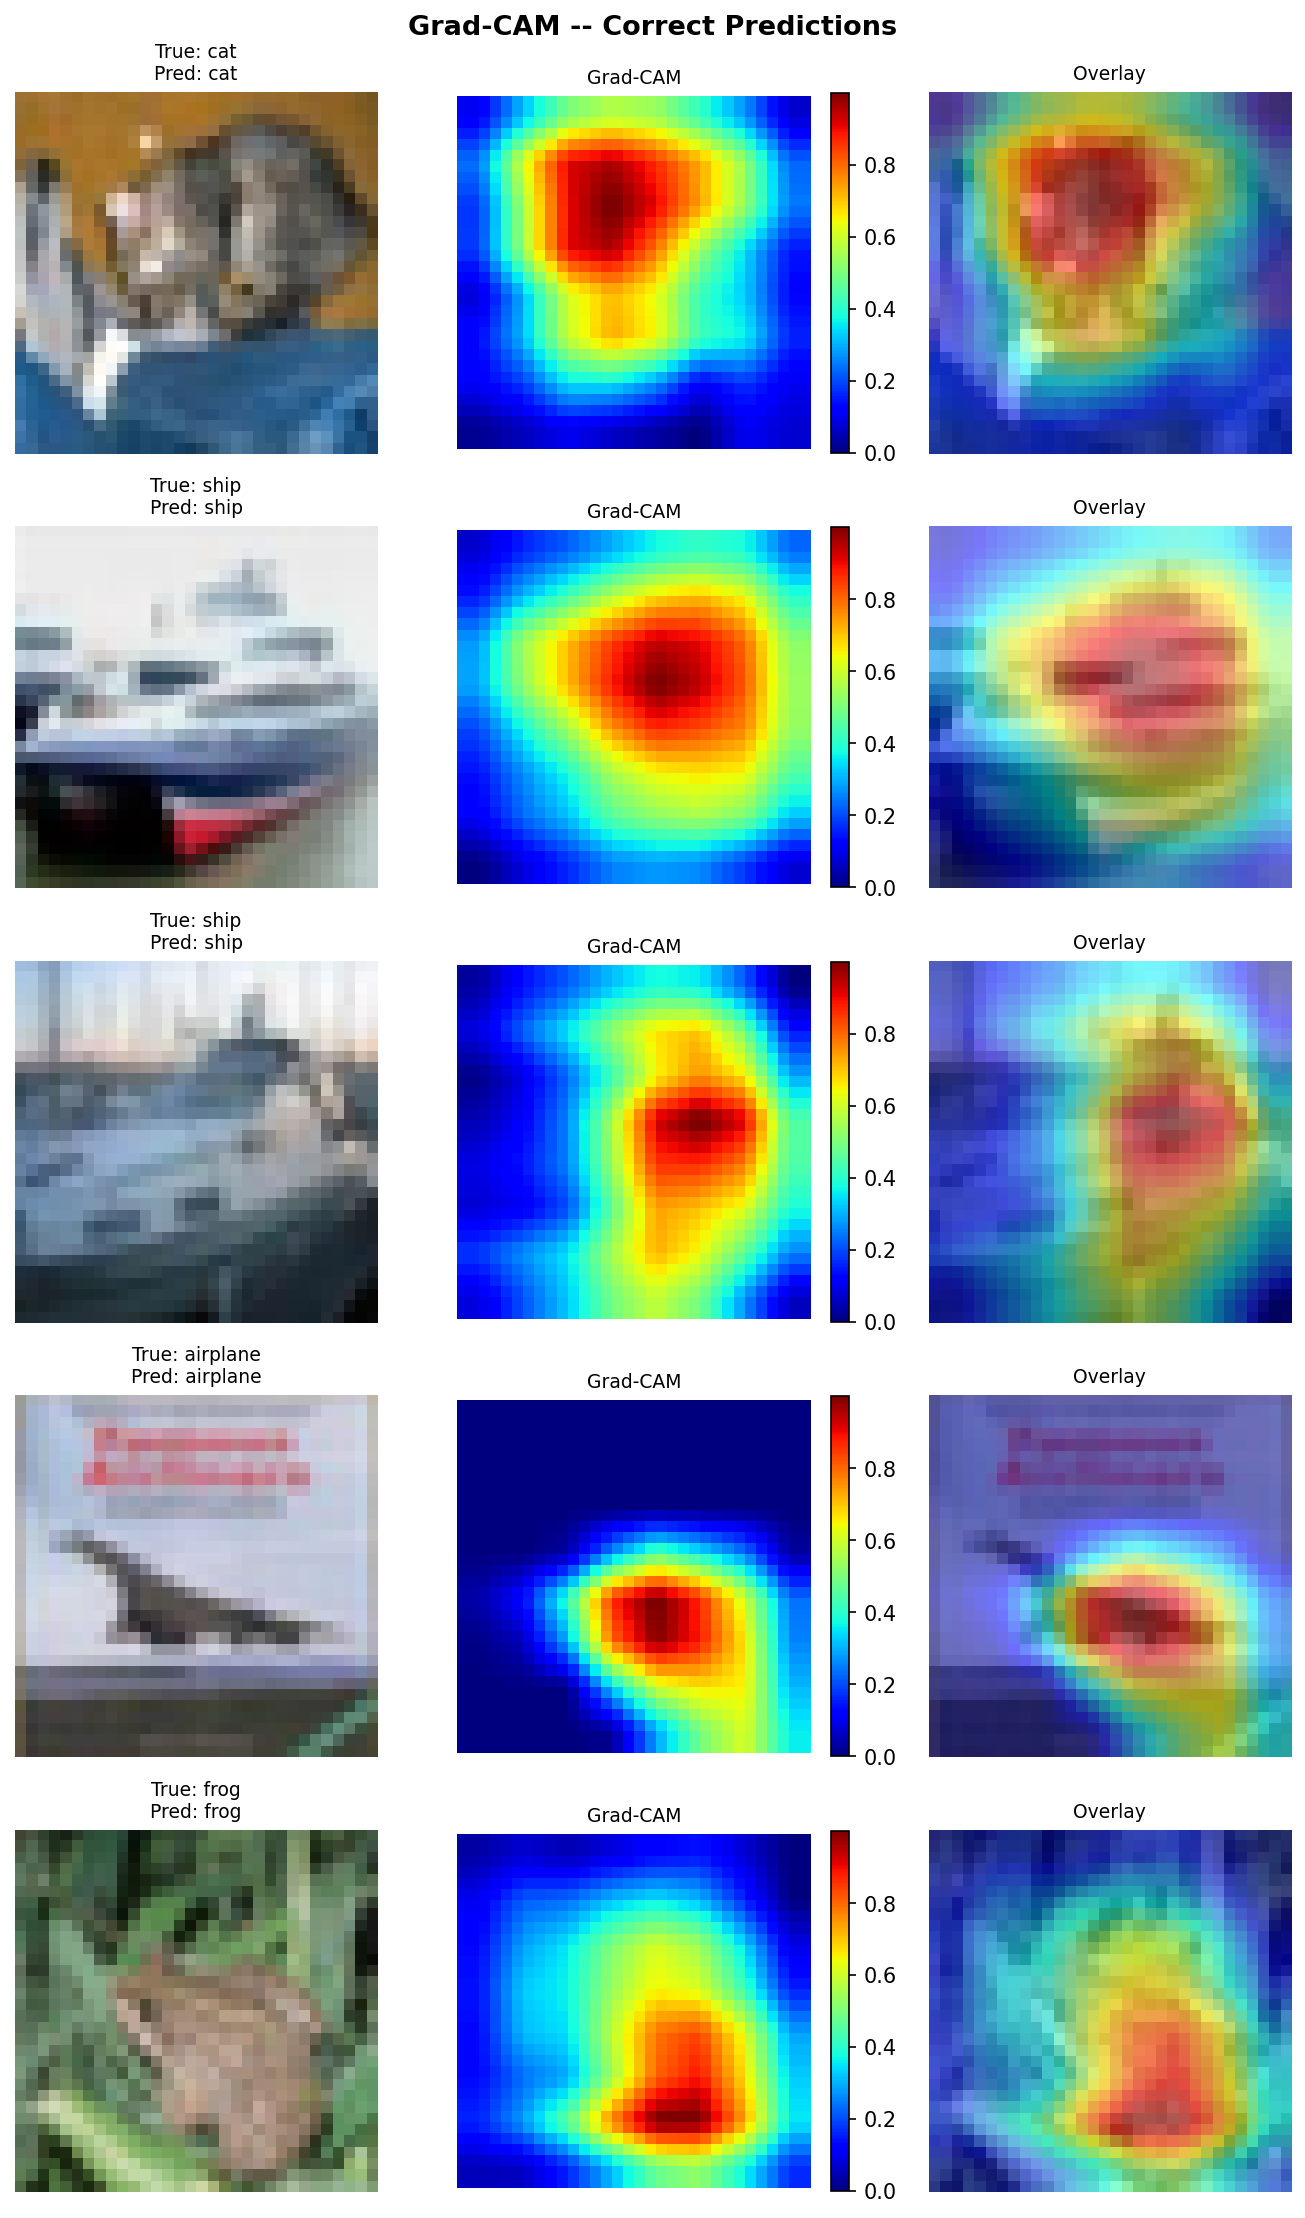
\includegraphics[width=0.85\textwidth]{gradcam_correct.png}
\caption{Grad-CAM heatmaps for correct predictions.}
\end{figure}

Grad-CAM heatmaps for correct predictions consistently highlight the object region. Compared to occlusion sensitivity, Grad-CAM produces smoother, more localised activations because it operates on the coarse spatial resolution of the final feature maps ($8\times8$) rather than pixel-level perturbations. This also makes Grad-CAM significantly faster -- a single backward pass versus hundreds of forward passes for occlusion.

\begin{figure}[H]
\centering
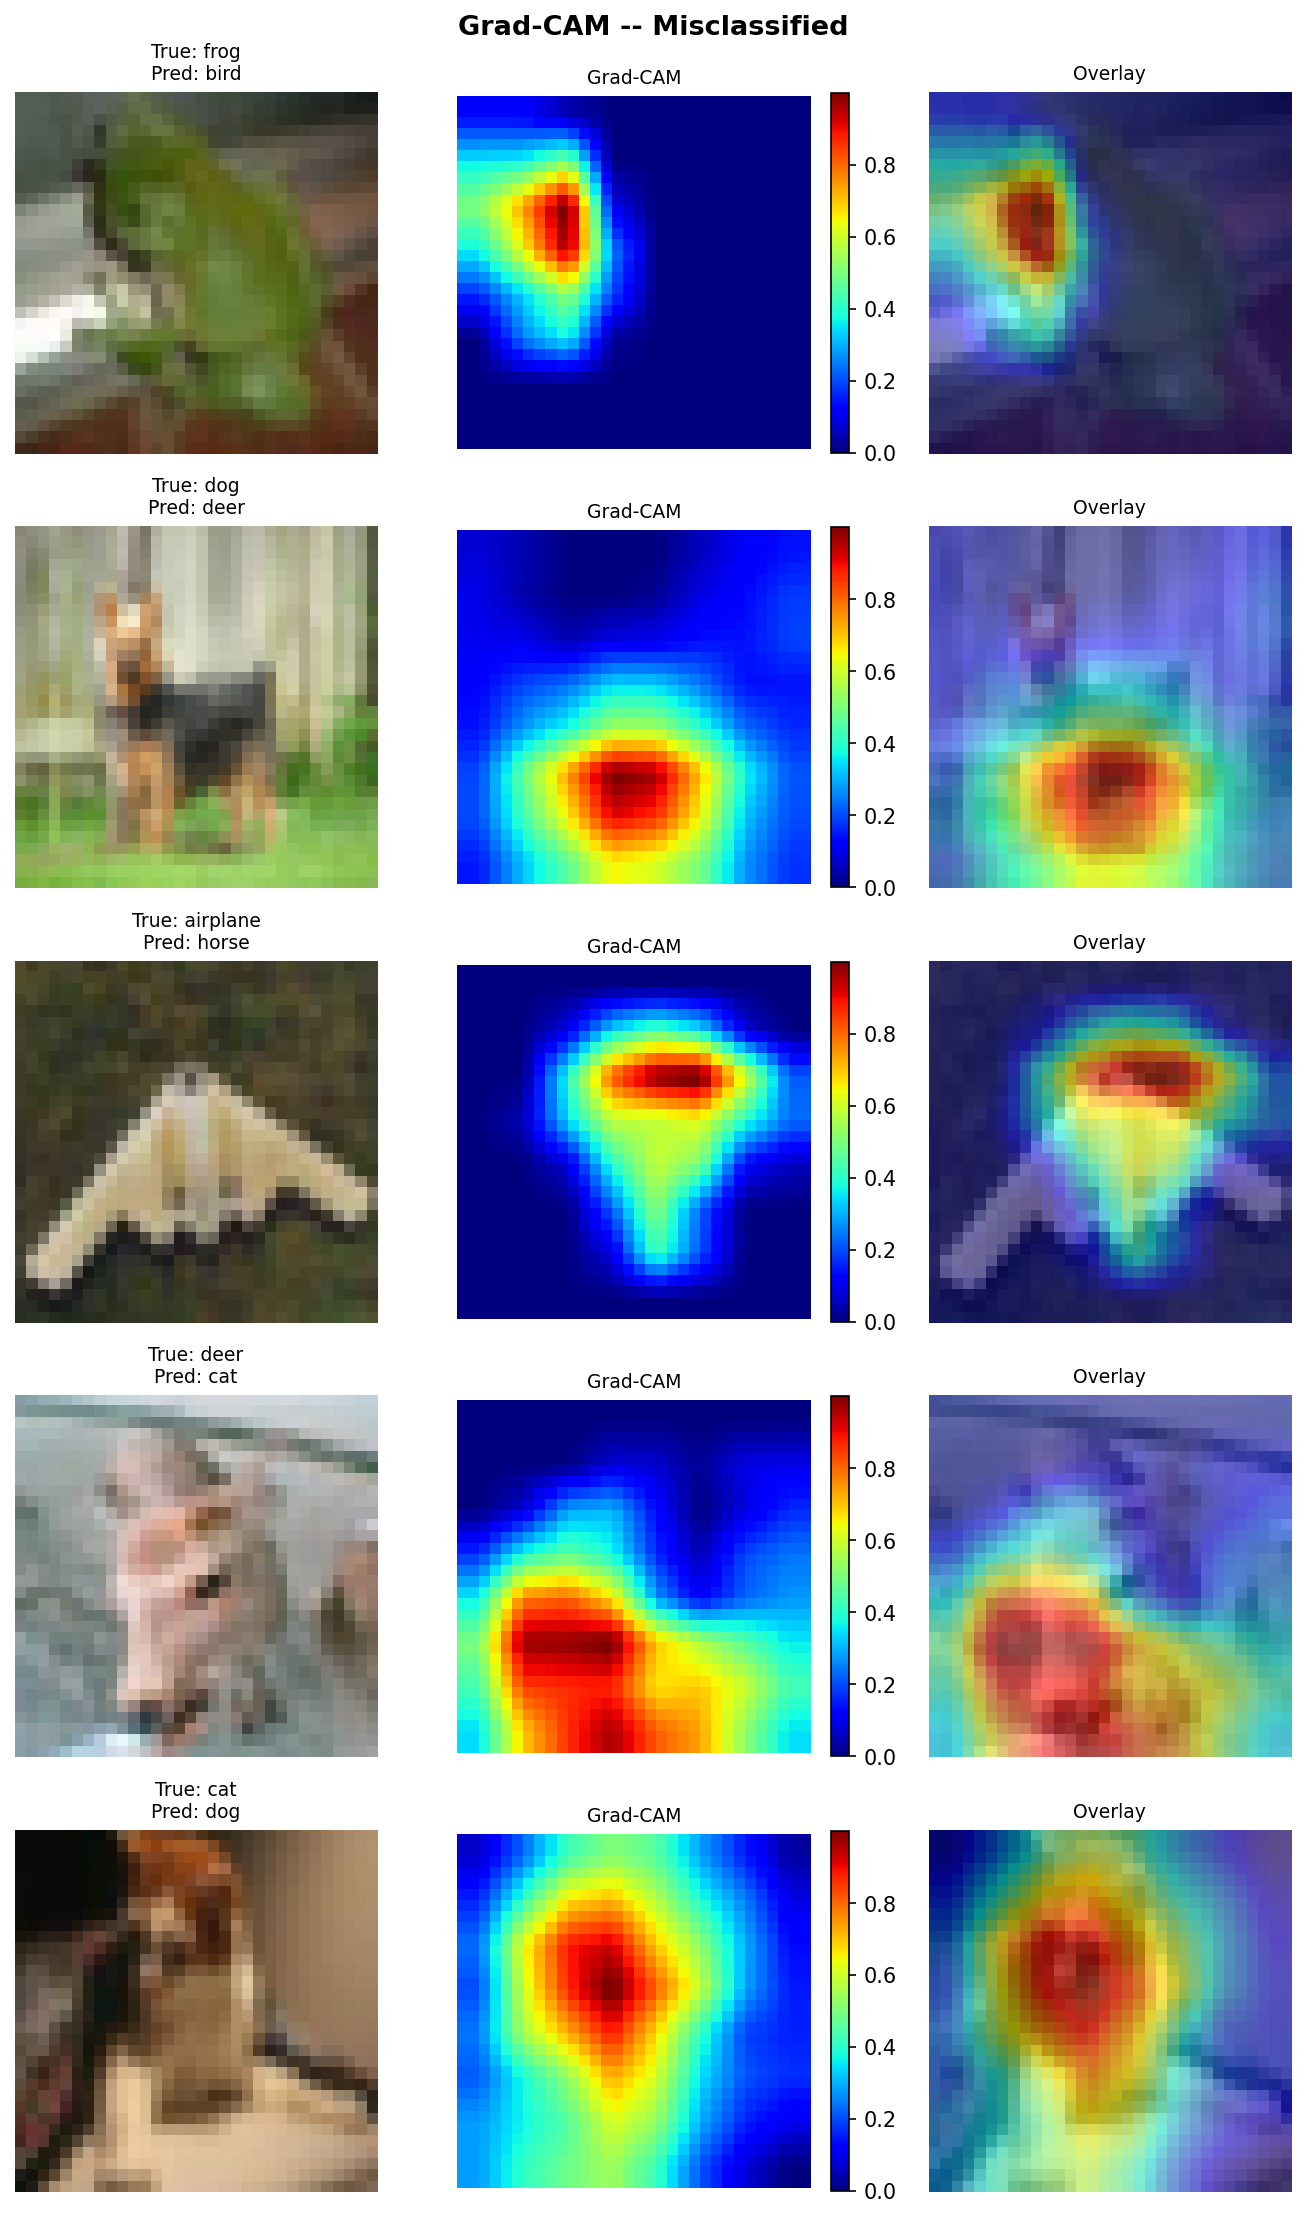
\includegraphics[width=0.85\textwidth]{gradcam_incorrect.png}
\caption{Grad-CAM heatmaps for misclassified images.}
\end{figure}

For misclassified images, Grad-CAM reveals the model attending to misleading regions -- for example, focusing on background texture rather than the object, or activating on a small region that resembles the predicted (wrong) class. This is consistent with the occlusion findings but provides a more spatially precise view.

\section{Part C: LIME}

LIME (Local Interpretable Model-agnostic Explanations) explains individual predictions by perturbing superpixels, observing prediction changes, and fitting a local linear model. Unlike Grad-CAM, LIME is model-agnostic -- it treats the classifier as a black box.

\begin{figure}[H]
\centering
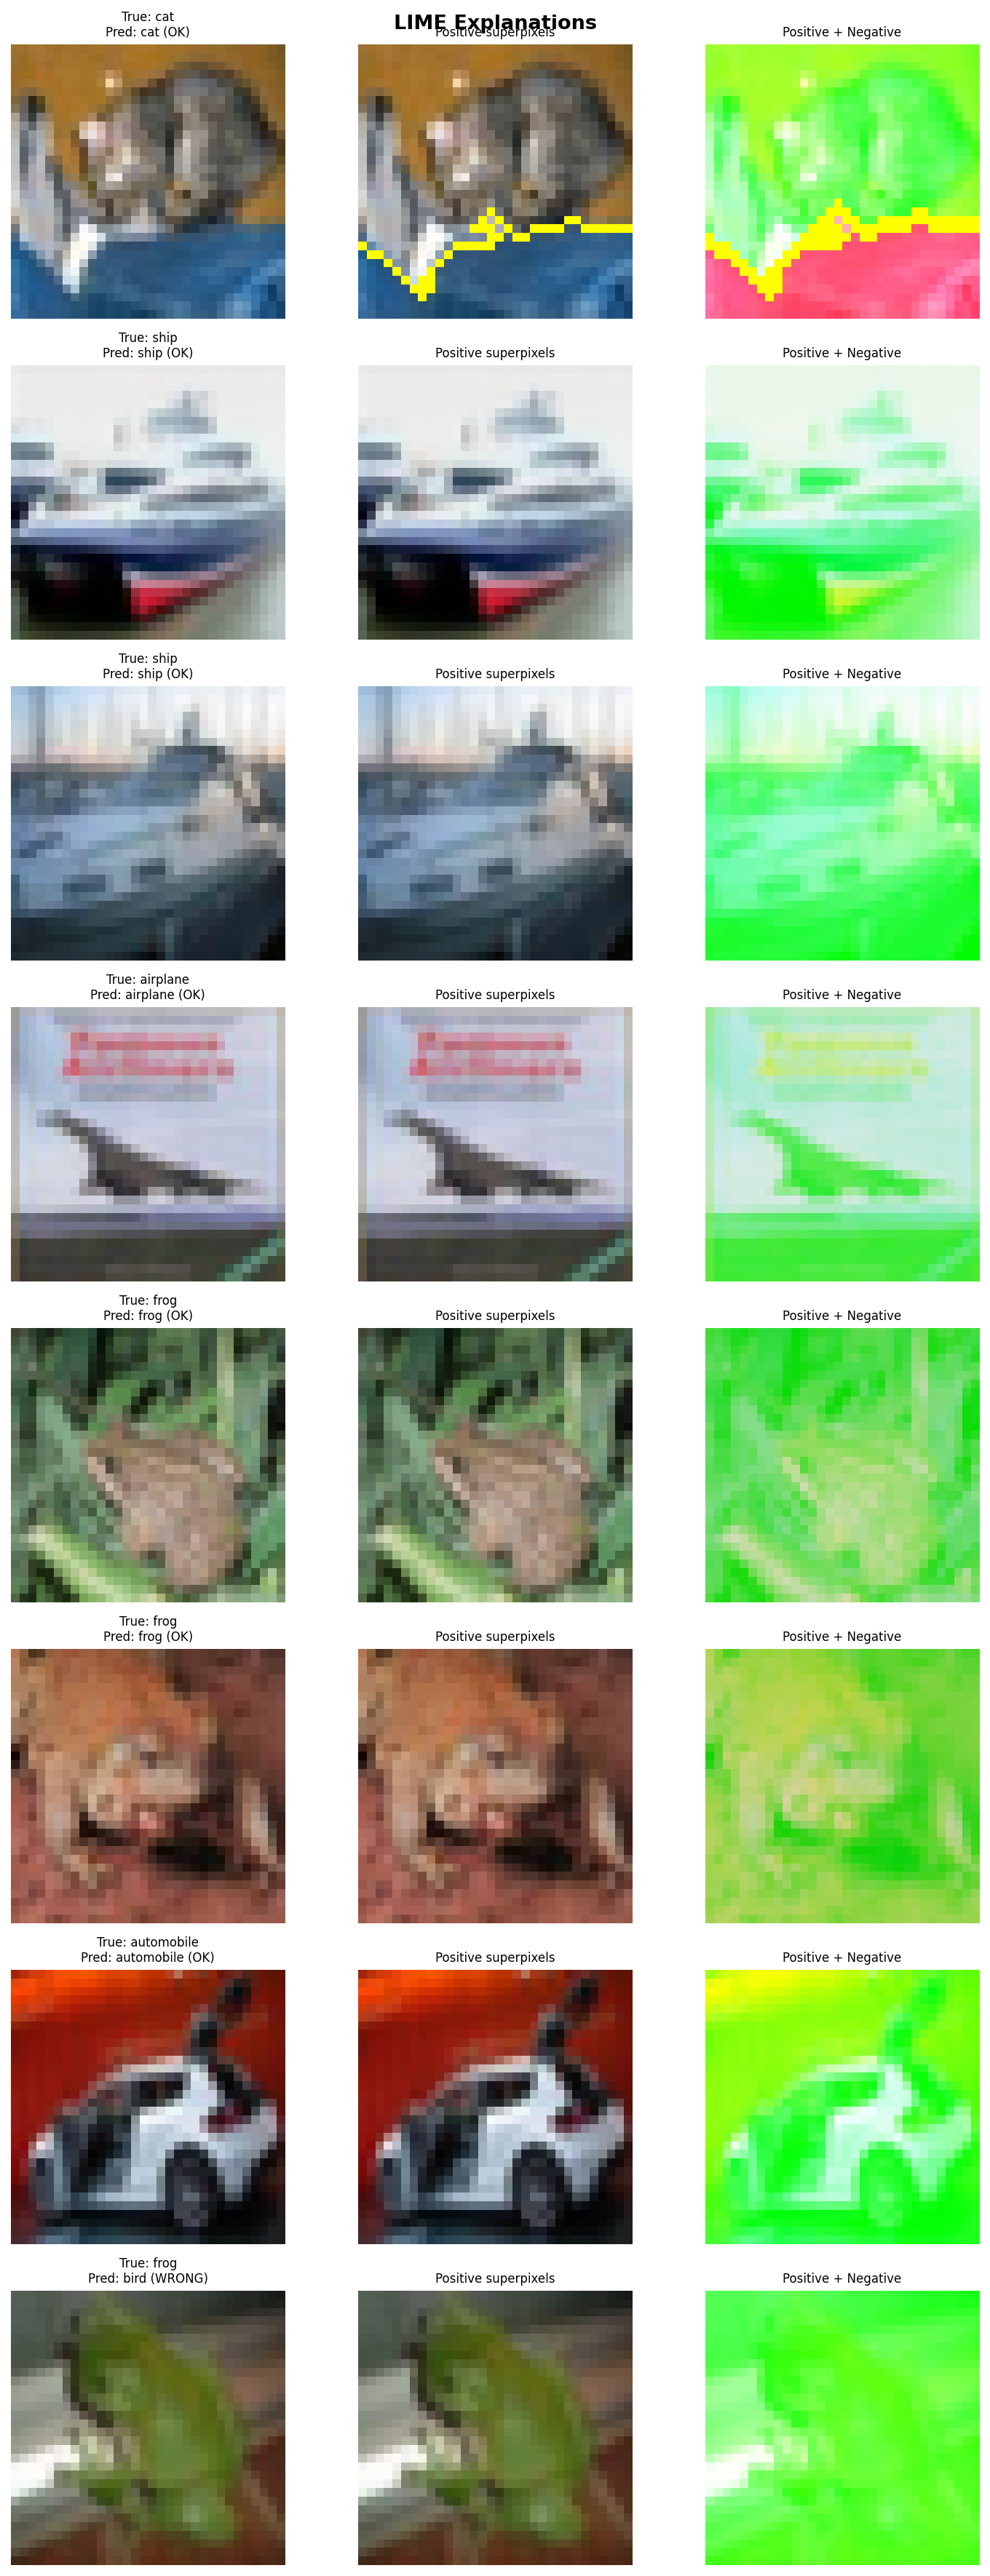
\includegraphics[width=0.85\textwidth]{lime_explanations.png}
\caption{LIME explanations showing positive superpixels (supporting the prediction) and positive+negative regions.}
\end{figure}

LIME identifies superpixel regions that support (green boundaries) or contradict (red boundaries) the prediction. For correct predictions, the positive superpixels cover the object. For the misclassified image (frog predicted as bird), LIME shows the model relying on background superpixels, consistent with occlusion and Grad-CAM findings. A limitation on $32\times32$ images is that superpixels are coarse relative to image size, making explanations less precise than on higher-resolution data.

\section{Part D: SHAP}

\textbf{D1 -- Titanic (tabular).} We computed SHAP values using TreeExplainer on a Random Forest classifier (79.0\% accuracy). Sex and Fare are the two most important features globally, followed by Age and Pclass. Being male strongly pushes survival probability down, while higher fare pushes it up -- consistent with historical accounts of women and upper-class passengers being prioritised during evacuation.

\begin{figure}[H]
\centering
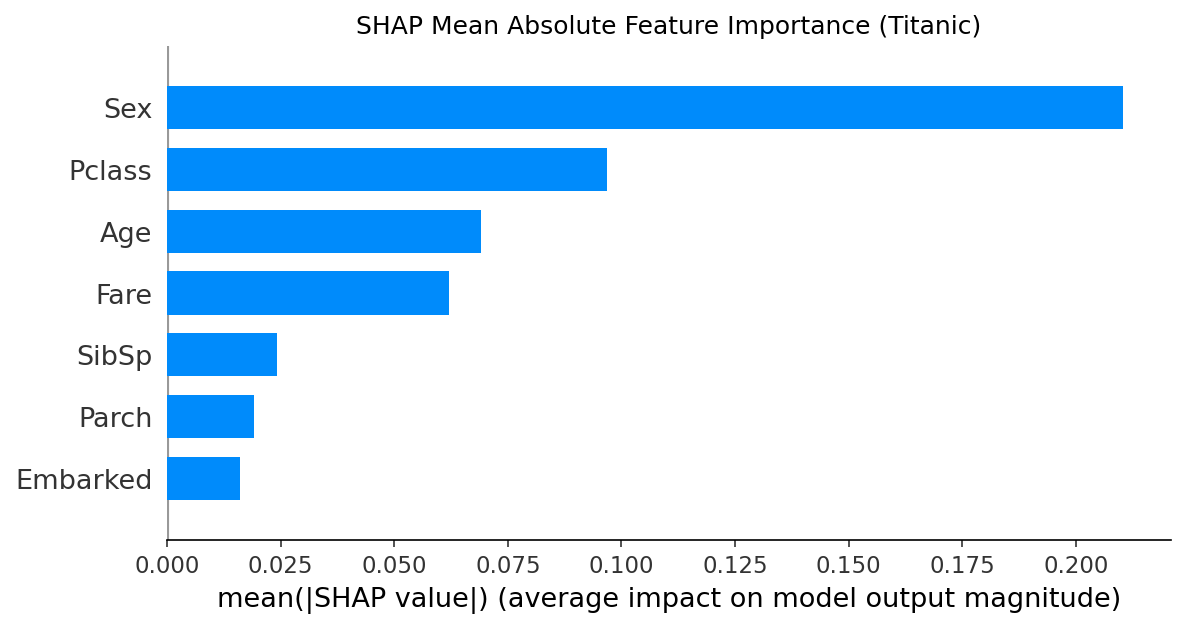
\includegraphics[width=0.7\textwidth]{shap_titanic_bar.png}
\caption{SHAP mean absolute feature importance for Titanic survival prediction.}
\end{figure}

\textbf{D2 -- CIFAR-10 (images).} We used SHAP's Partition Explainer with inpainting masking to compute pixel-wise Shapley values. Red regions contribute positively to the predicted class; blue regions contribute negatively.

\begin{figure}[H]
\centering
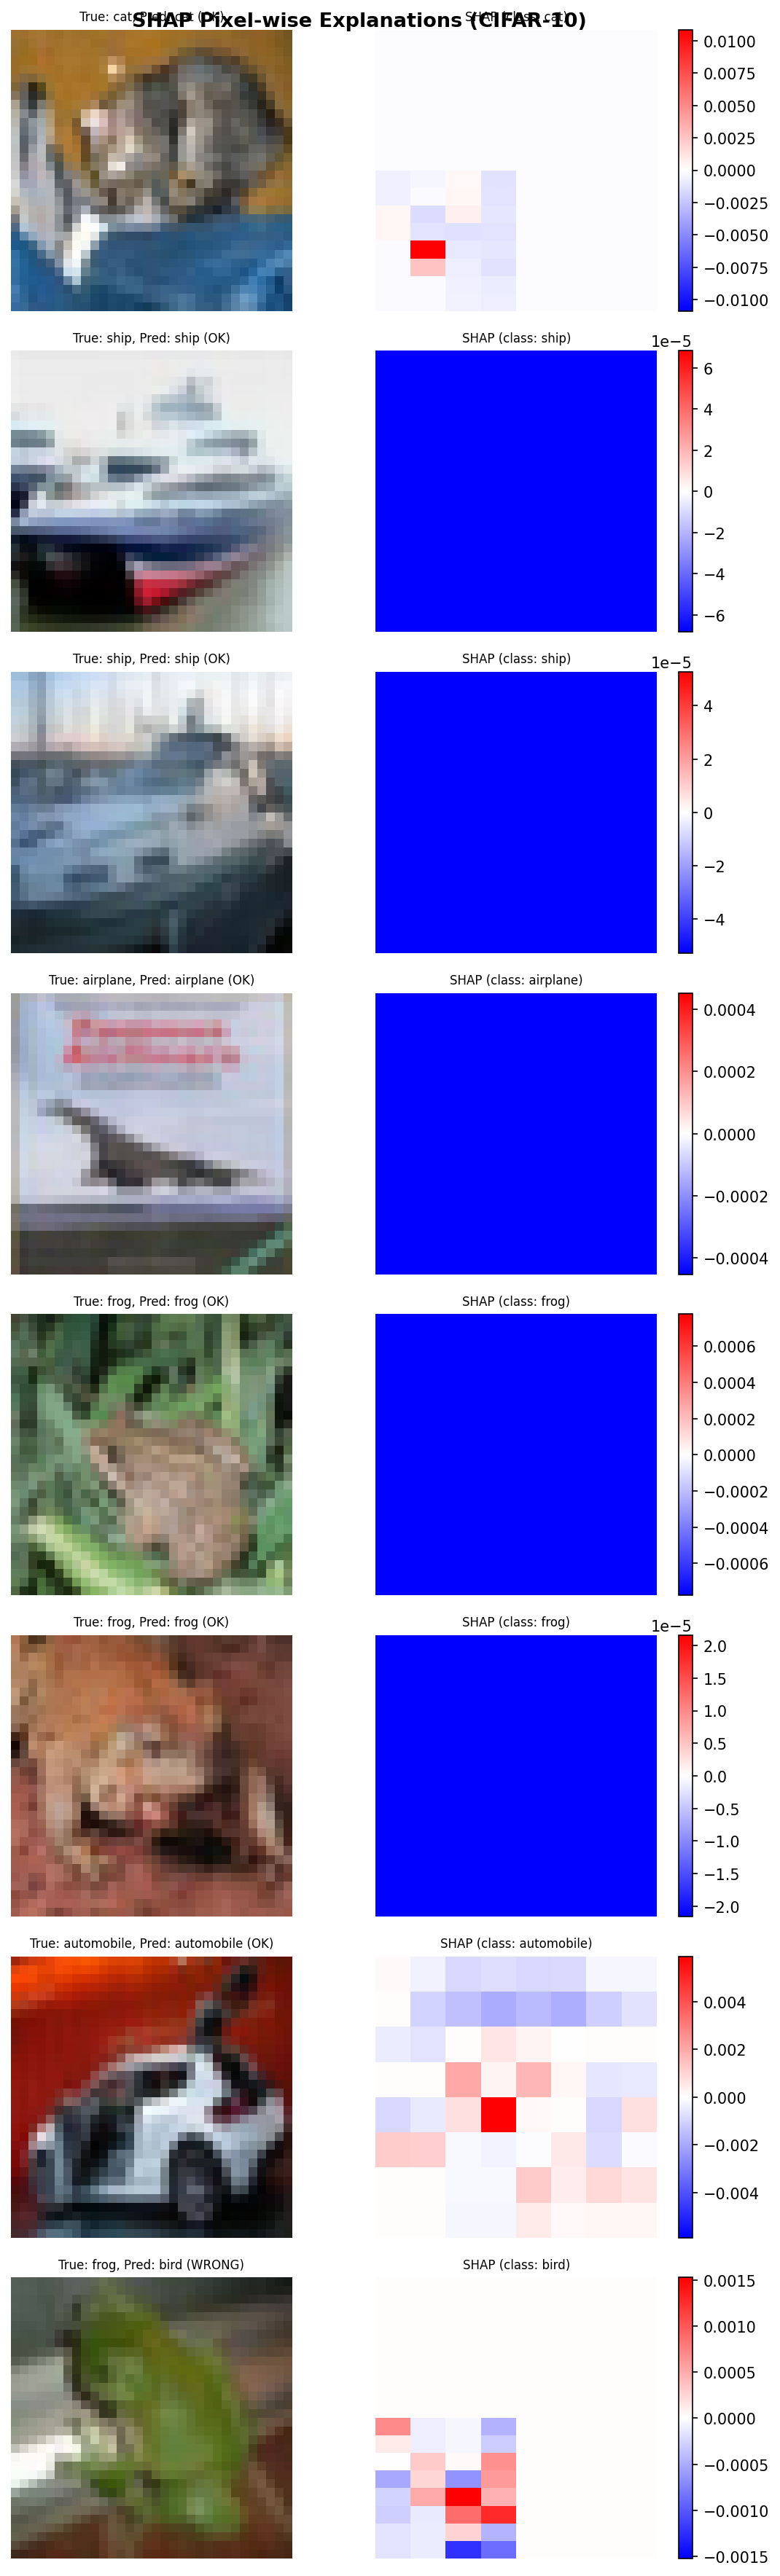
\includegraphics[width=0.75\textwidth]{shap_cifar10_images.png}
\caption{SHAP pixel-wise explanations for CIFAR-10 images. Red = positive contribution, blue = negative.}
\end{figure}

The SHAP image explanations are noisier than Grad-CAM but provide a principled, model-agnostic attribution with theoretical guarantees (additivity, symmetry, dummy). On small images, the computational cost is manageable (500 evaluations per image), but on larger images SHAP becomes prohibitively expensive, which is a practical limitation compared to gradient-based methods.

\end{document}
